\documentclass[tikz,border=6pt]{standalone}
\usetikzlibrary{arrows.meta}
\definecolor{red}{HTML}{A50F2D}\definecolor{ink}{HTML}{141414}\definecolor{gry}{HTML}{5F5F5F}
% double well: local minimum (left), high barrier (middle), deeper global minimum (right)
\newcommand{\curve}{\draw[ink,very thick,smooth,samples=100,domain=0.1:3.9] plot (\x,{0.75*(0.5*(\x-2)^4-2.2*(\x-2)^2-0.45*(\x-2)+3.1)+0.15});}
\newcommand{\barrier}{\draw[gry,dashed] (1.9,2.49) -- (1.9,3.0); \node[gry,font=\sffamily\small] at (1.9,3.2) {barrier};}
\begin{document}
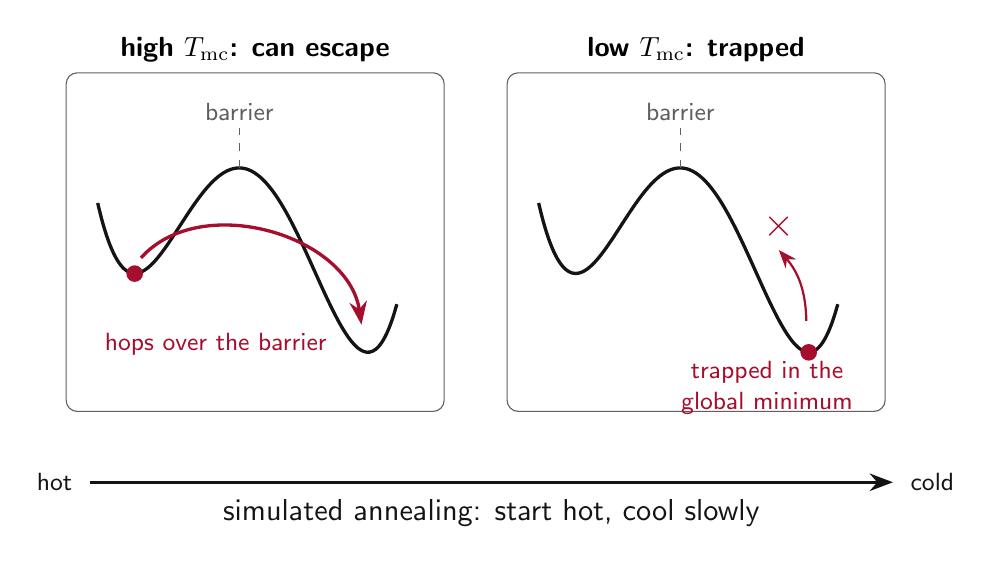
\begin{tikzpicture}[font=\sffamily\fontsize{11}{13}\selectfont,>=Stealth]
% high T panel: start of the annealing, the particle sits in the shallow minimum and can cross the barrier
\draw[gry,rounded corners] (-0.3,-0.6) rectangle (4.5,3.7);
\node[font=\sffamily\bfseries] at (2.1,4.0) {high $T_{\mathrm{mc}}$: can escape};
\curve \barrier
\fill[red] (0.57,1.15) circle (3pt);
\draw[red,very thick,->] (0.65,1.35) to[bend left=65] (3.45,0.5);
\node[red,font=\sffamily\small] at (1.6,0.25) {hops over the barrier};
% low T panel: end of the annealing, the particle is trapped in the global minimum
\begin{scope}[xshift=5.6cm]
\draw[gry,rounded corners] (-0.3,-0.6) rectangle (4.5,3.7);
\node[font=\sffamily\bfseries] at (2.1,4.0) {low $T_{\mathrm{mc}}$: trapped};
\curve \barrier
\fill[red] (3.53,0.15) circle (3pt);
\draw[red,thick,->] (3.5,0.55) to[bend right=20] (3.15,1.45);
\node[red,font=\sffamily\bfseries\Large] at (3.15,1.75) {$\times$};
\node[red,font=\sffamily\small,align=center] at (3.0,-0.3) {trapped in the\\global minimum};
\end{scope}
% annealing arrow
\draw[->,ink,very thick] (0.0,-1.5)--(10.2,-1.5);
\node[ink,anchor=north] at (5.1,-1.6) {simulated annealing: start hot, cool slowly};
\node[ink,font=\sffamily\small,anchor=east] at (-0.1,-1.5) {hot};
\node[ink,font=\sffamily\small,anchor=west] at (10.3,-1.5) {cold};
\end{tikzpicture}
\end{document}
